\chapter{He Made \$7M/Year and Paid Zero Taxes!}

These notes follow a School of Hard Knocks interview with Carlton Dennis, arranged here as a companion chapter curated by LazyingArt LLC. The lecture begins with spectacle, but it does not stay there. Very quickly the Ferrari becomes a numerical puzzle, and the puzzle becomes a study of how income, legal structure, depreciation, leverage, and timing interact. The right way to read the interview is not as a list of hacks, but as a sequence: first the paradox, then the lawful mechanisms, then the simpler moves for early operators, then the worked example that finally puts arithmetic on the board.

\section{The Opening Puzzle}

We begin with the headline quantities, because the lecture itself begins there. Dennis is introduced not simply as an entrepreneur with expensive cars, but as an entrepreneur who claims very high annual income with very low taxes. The numbers are the first source of tension:

\begin{align}
Y_{2023} &\approx \$7.1\,\text{million}, &
Y_{2024} &\approx \$11.5\,\text{million}, \\
T_{\mathrm{fed},2023} &= \$0, &
T_{\mathrm{state},2023} &= \$26{,}000, \\
T_{\mathrm{total},2024} &< \$92{,}000. &&
\end{align}

The host quite properly treats this as a paradox. If the income scale is this large, then how can the tax bill remain this small? The lecture needs this paradox, because without it there is no reason to care about the machinery that follows.

\subsection{Question \& Answer}

\paragraph{Question.} How can somebody earn millions and still pay almost nothing in taxes without breaking the law?

\paragraph{Answer.} Dennis answers this immediately in the language of legality. He insists that the game is played ``by the book,'' and he compresses his method into three recurring mechanisms:
\begin{equation}
\text{tax reduction}
\to
\{\text{income shifting},\ \text{depreciation},\ \text{philanthropy}\}.
\end{equation}
This is the first structural move of the lecture. The puzzle is not answered by denial or concealment; it is answered by saying that taxable income can be lawfully altered through the form in which income appears, the timing of deductions, and the placement of capital.

\section{Why Taxes Become the Real Expense}

The lecture then broadens from Dennis's own case to the ordinary business owner. This is an important transition. We are told that the largest expense for many operators is not the mortgage, not the car payment, and not payroll, but taxes themselves. The lecture's warning is simple: people often go broke not because they failed to earn, but because they spent the portion of cash that should eventually have gone to the government.

From here Dennis gives the first strong mechanism. If one is earning W-2 or 1099 income, then short-term rentals enter as a candidate tax machine:

\begin{equation}
\text{cost segregation}
\Rightarrow
\text{paper loss}
\Rightarrow
\text{offset W-2 / 1099 income}.
\end{equation}

The local conditions are stated in the interview in practical rather than symbolic language:
\begin{equation}
\mathrm{STR}=7\ \text{days or less},
\qquad
\text{manage for }100\ \text{hours}.
\end{equation}

The logic is clear even before the numbers appear. If the property is short-term enough, and if the management participation is sufficient, then the rental is no longer being described as a passive sideline in the lecture. It becomes an active business context within which accelerated depreciation can create a current paper loss. The same idea is then extended to a household arrangement: if one spouse is not otherwise working, Dennis presents that spouse as the natural candidate to manage the real-estate portfolio and thereby strengthen the active-business posture of the real-estate side.

\section{Early Structure Before Big Assets}

The host then asks the necessary corrective question. What about the operator who is not yet in position to buy a rental property? The lecture does not ignore this objection. It backs up and gives the earlier structural moves.

The first move is entity structuring. Dennis places a threshold near the point where self-employed income crosses roughly \$50{,}000 to \$60{,}000:
\begin{equation}
I_{\text{self-employed}} \gtrsim \$50{,}000\text{--}\$60{,}000
\Rightarrow
\text{consider S-corporation treatment}.
\end{equation}

He then states the relevant burden in plain terms:
\begin{equation}
\tau_{\mathrm{SE}} = 15.3\%.
\end{equation}

A cleaned lecture-level formulation of his claim is
\begin{align}
T_{\mathrm{SE,sole\ prop}} &\approx \tau_{\mathrm{SE}}\Pi, \\
T_{\mathrm{SE,S\ corp}} &\approx \tau_{\mathrm{SE}}S,
\end{align}
where \(\Pi\) denotes business profit and \(S\) the owner salary. This is not a full legal derivation of payroll and self-employment taxation; it is the algebraic skeleton of the point made in the interview. The burden that initially hits all of profit is, after the structural change, said to hit the salary component rather than the entire remaining pool.

\subsection{Question \& Answer}

\paragraph{Question.} Why does the S-corporation threshold matter once a self-employed person crosses roughly \$50{,}000 to \$60{,}000?

\paragraph{Answer.} Because the lecture treats that threshold as the point where entity form begins to matter materially. Below it, the simplicity of the original structure may dominate. Above it, the difference between taxing all profit and taxing only the salary component becomes large enough to justify the added complexity. The threshold is therefore pedagogical as much as legal: it marks the point where structure ceases to be bookkeeping and starts to become strategy.

The second move is much less glamorous and therefore easy to overlook. Dennis insists that many business owners have already spent money on deductible business uses without classifying it correctly. The chapter should preserve that prosaic point. The lecture treats deduction capture as an operator discipline. Cell phones, laptops, and business travel wrongly left on a personal card are not a new source of wealth, but they can still reduce taxable income by correcting the accounting boundary.

\section{Speed and the Difference Between Planning and Paying}

At this point the lecture turns from structure to temperament. This is not filler. Dennis says the difference between wealthy operators and middle-class earners is often speed. The wealthy do not merely ask whether a tax-reducing move is possible; they ask where to move the money, when to wire it, and how quickly the structure can be put in place. The middle class, in his telling, becomes trapped in analysis paralysis.

This part of the lecture is easy to misread as psychology. It is more concrete than that. The claim is that tax planning is time-sensitive. The person who is willing to deploy money into vehicles, foundations, properties, or entities before the tax year closes can still alter the shape of taxable income. The person who hesitates eventually pays in cash what he would rather have paid in structure.

The host then asks for scale, and Dennis answers with a very large one: he claims to have saved clients well over \$100 million in taxes. Whether or not one lingers on the size of that figure, the narrative function is obvious. We are being moved from doctrine to proof by example.

\section{Cases, Cars, and Leverage}

The first large example is the yacht audit. Its importance is not the yacht itself. Its importance is that Dennis uses it to show that documentation is inseparable from deduction. He describes a client whose claimed deduction was challenged, and he says the defense rested on records: captain's logs, photographs, and the profit-and-loss trail. He also states the operative standard in words: ordinary, necessary, and reasonable business expense in pursuit of income. It is best to preserve that standard without leaning too heavily on the exact statute citation, because the transcript's numeric code reference is not entirely secure.

The lecture then moves outside again, now to vehicles. Here the car ceases to be a toy and becomes a tax object. Dennis says one vehicle generated about \$92{,}000 in tax savings, and that the savings were rolled into a multifamily property producing about \$1{,}400 per month in cash flow:
\begin{equation}
\Delta T_{\mathrm{G\text{-}Wagon}} \approx \$92{,}000
\to
\text{multifamily reinvestment}
\to
\$1{,}400/\text{month}.
\end{equation}

He then states the eligibility logic for the heavy-vehicle write-off:
\begin{equation}
\mathrm{GVWR} > 6{,}000\ \text{lb},
\qquad
u_{\mathrm{biz}} > 50\%.
\end{equation}
The deduction is described in the interview through the combination
\begin{equation}
\text{Section }179 + \text{Section }168\mathrm{K},
\end{equation}
together with an internal timeline for bonus depreciation:
\begin{equation}
b_{2023}=80\%,
\qquad
b_{2024}=60\%.
\end{equation}
Dennis also speculates that bonus depreciation may return to \(100\%\). In these notes we record that as a lecture-side expectation, not as a theorem we ourselves are using.

\subsection{Question \& Answer}

\paragraph{Question.} How can a depreciating asset or a debt-financed purchase still improve the operator's financial position?

\paragraph{Answer.} Because the lecture is not comparing the car to holding no asset at all. It is comparing one cash path to another. Dennis's example is:
\begin{align}
I &= \$200{,}000, \\
E_{\mathrm{down}} &= \$20{,}000, \\
W &\approx \$200{,}000, \\
T_{\mathrm{counterfactual}} &\approx \$50{,}000.
\end{align}
If the write-off neutralizes the taxable income, then the lecture invites us to compare the avoided tax to the down payment:
\begin{equation}
\$50{,}000 - \$20{,}000 = \$30{,}000.
\end{equation}
The claim is not that the car becomes an appreciating asset. The claim is that the tax savings and the redeployment of those savings can outweigh the immediate cash required to acquire the vehicle.

From there the lecture widens into leverage. Dennis distinguishes bad debt from good debt:
\begin{equation}
\text{consumer debt}\to \text{bad debt},
\qquad
\text{asset-backed leverage}\to \text{good debt}.
\end{equation}
He then voices two heuristics that matter for the chapter's conceptual spine:
\begin{equation}
D\uparrow \Rightarrow \text{buying power}\uparrow,
\qquad
\text{wealth}\sim \text{access to debt}.
\end{equation}
These are not strict identities. They are rules of operator behavior. Debt is being treated not simply as obligation but as scale. Real estate becomes the model case because leverage can enlarge the portfolio while refinances and HELOCs can re-release capital, and inheritance can eventually transfer the accumulated portfolio after the debt work has already done its job.

\section{The Board Example: A \$500{,}000 Property and a \$100{,}000 Paper Loss}

Only late in the lecture do we finally reach the board. This is where the verbal theory is forced into arithmetic.

\begin{figure}[h]
\centering

\includegraphics[width=0.82\textwidth]{lecture_56_figure_03.png}
\end{figure}

The original screenshot should remain here because the board itself is evidence. We can see the short-term-rental condition, the \(100\)-hour management requirement, the cost-segregation label, and the final \(\$100{,}000\) payoff, even though part of the writing is blocked.

\begin{figure}[h]
\centering
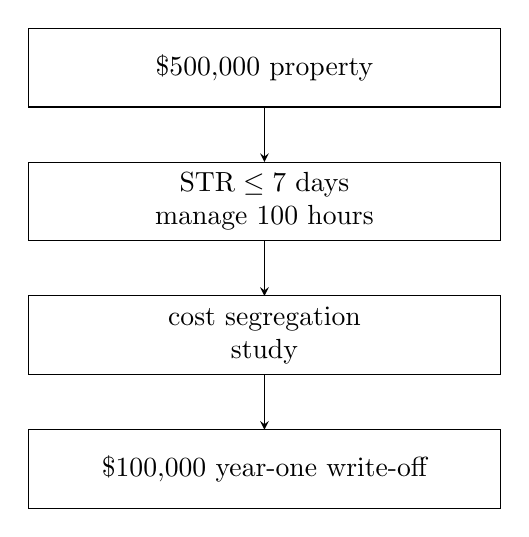
\begin{tikzpicture}[>=stealth]
\draw (-3,6) rectangle (3,7) node[pos=.5]{\(\$500{,}000\) property};
\draw (-3,4.3) rectangle (3,5.3) node[pos=.5]{\shortstack{\(\mathrm{STR}\le 7\) days\\manage \(100\) hours}};
\draw (-3,2.6) rectangle (3,3.6) node[pos=.5]{\shortstack{cost segregation\\study}};
\draw (-3,0.9) rectangle (3,1.9) node[pos=.5]{\(\$100{,}000\) year-one write-off};
\draw[->] (0,6) -- (0,5.3);
\draw[->] (0,4.3) -- (0,3.6);
\draw[->] (0,2.6) -- (0,1.9);
\end{tikzpicture}
\end{figure}

\subsection{Question \& Answer}

\paragraph{Question.} How does a \$500{,}000 property become a \$100{,}000 paper loss?

\paragraph{Answer.} The lecture answers by a short worked chain. We preserve it in cleaned form, but we also keep the visual evidence nearby because the board itself is partially occluded.

\begin{enumerate}
\item Start with an operator earning
\[
I_{\mathrm{W2}}=\$100{,}000.
\]

\item Acquire a property with purchase price
\[
P_{\mathrm{prop}}=\$500{,}000
\]
using
\[
E_{\mathrm{down}}=\$100{,}000,
\qquad
L_{\mathrm{loan}}=\$400{,}000.
\]

\item Place the property into short-term-rental use with the lecture's two local conditions:
\[
\mathrm{STR}=7\ \text{days or less},
\qquad
\text{manage for }100\ \text{hours}.
\]

\item Perform a cost segregation study and use the lecture's rule of thumb
\[
W_{1}=20\%\cdot P_{\mathrm{prop}}.
\]

\item Compute the year-one write-off:
\[
W_{1}=0.20\times \$500{,}000=\$100{,}000.
\]

\item Match that paper loss against the initial income:
\[
I_{\mathrm{W2}}=\$100{,}000,
\qquad
L_{\mathrm{paper}}=\$100{,}000
\Rightarrow
T\approx 0
\]
in the example presented.
\end{enumerate}

\paragraph{Caveat.} The board is not perfectly legible. The \(\$500{,}000\) input and the exact bottom line are partially obscured. The cleaned equation above is therefore a cautious reconstruction guided by the visible layout and by the spoken statement that the result is \(\$100{,}000\). But the logic of the example is stable: a leveraged property purchase is converted, through short-term-rental classification and cost segregation, into a year-one paper loss large enough to offset the income being discussed.

The lecture then immediately expands the example by scale. If the same game is played with a larger property and larger income, the same percentage logic can be carried upward. That is why Dennis returns once more to debt. One does not need the full price of the asset in cash; one needs enough equity to control the asset and enough structure to produce the deduction.

\section{The Augusta Rule}

The lecture closes with a final portable rule. Dennis tells the origin story through Augusta, Georgia, and then states the threshold that matters:
\begin{equation}
d_{\mathrm{Augusta}} \le 14\ \text{days}.
\end{equation}
He names the federal reference as
\begin{equation}
\mathrm{IRC}\text{-}280\mathrm{A}.
\end{equation}

The key point is that the first \(14\) days of rental income can, in the lecture's presentation, be received without tax. Dennis then folds that rule back into the S-corporation framework.

\subsection{Question \& Answer}

\paragraph{Question.} Why does the Augusta Rule function like a tax-free distribution back to the owner?

\paragraph{Answer.} Because the lecture treats the S corporation and the owner as distinct parties for this purpose. The chain is:
\begin{equation}
\text{owner} \leftrightarrow \text{S corp}
\to
\text{rent residence for }14\text{ days}
\to
\text{deduction at S-corp level + tax-free rent to owner}.
\end{equation}

We may write the lecture's logic as a sequence:
\begin{enumerate}
\item The owner controls an S corporation.
\item The S corporation rents the owner's primary residence for a limited number of days.
\item The rent is deductible to the corporation.
\item The owner receives the rent under the lecture's \(14\)-day tax-free window.
\end{enumerate}

This is why Dennis calls it low-hanging fruit. It is not the lecture's largest mechanism, but it is its cleanest final example: a named rule, a clear threshold, and a short loop from entity to individual.

\section{Summary}

The lecture begins with a paradox and ends with a toolkit. First come the big numbers, because the puzzle must be visible before the method matters. Then come the three broad mechanisms: income shifting, depreciation, and philanthropy. After that, the interview moves carefully between scales. It gives the large real-estate paper-loss idea, backs up to simpler entity-structure moves for the earlier operator, insists on speed as a practical difference between those who plan and those who merely worry, and then tests the claims through cases involving audits, vehicles, reinvestment, and leverage.

The mathematical center of the chapter is the whiteboard example. There the interview finally slows down enough for us to see the lecture's preferred arithmetic:
\[
0.20\times \$500{,}000=\$100{,}000.
\]
Everything around it prepares that line. And everything after it compresses the lesson into a final rule: taxable outcomes are shaped not only by how much one earns, but by the form in which one earns, the deductions one can lawfully create, and the speed with which one acts before the year closes.